% !TeX spellcheck = es_ES
\documentclass[12pt, titlepage]{article}
\usepackage[utf8]{inputenc}
\usepackage[spanish]{babel}
\usepackage{float}
\usepackage[letterpaper, margin=2.5cm]{geometry}
\usepackage[nottoc,notlot,notlof]{tocbibind} % Hace que se agregen las referencias al indice
\usepackage{url}
\usepackage{graphicx} 
\usepackage{listings}
\usepackage{color}
\definecolor{dkgreen}{rgb}{0,0.6,0}
\definecolor{gray}{rgb}{0.5,0.5,0.5}
\definecolor{mauve}{RGB}{253,151,31}

\lstset{frame=tb,
	language=Sql,
	aboveskip=3mm,
	belowskip=3mm,
	showstringspaces=false,
	columns=flexible,
	basicstyle={\small\ttfamily},
	numbers=none,
	numberstyle=\tiny\color{gray},
	keywordstyle=\color{blue},
	commentstyle=\color{dkgreen},
	stringstyle=\color{mauve},
	breaklines=true,
	breakatwhitespace=true,
	tabsize=2,
	morekeywords={use}
}

\title{Reporte: Práctica 7}
\author{Carlos Tonatihu Barrera Pérez \\ Profesor: Hernández Contreras Euler \\ Bases de Datos \\ Grupo: 2CM1 }

\begin{document}
	\maketitle
	\tableofcontents
	\section{Marco Teórico}
	Supongo que estará con madre
	\section{Desarrollo}
	En esta práctica se llevaron a operaciones para modificar la información en la base de datos, es decir, se inserto nueva información y se ejecutaron eliminaciones.
	
	La primera operación que se llevó a cabo fue dar de alta a un socio y asignarlo a una sucursal determinada. Para realizar esto primero creamos un nuevo socio en la tabla socio. 
	\begin{lstlisting}
		insert into socio (idSocio,nombre,email,credito) values ("s1500","Hernandez Contreras Euler", "eulerelbonito@hotmail.com", 12000);
	\end{lstlisting}
	\begin{figure}[H]
		\begin{center}
			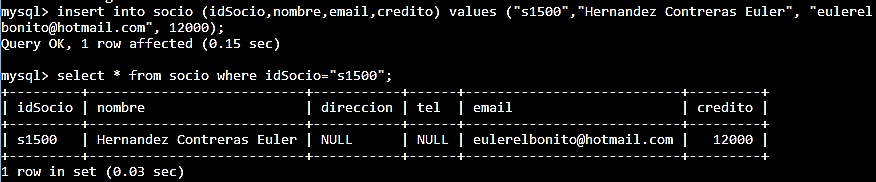
\includegraphics[width=\textwidth]{img/uno.png}
			\label{fig:uno}
		\end{center}
	\end{figure}
	Procedemos a asociarlo con una sucursal mediante la tabla hdsocio.
	\begin{lstlisting}
	insert into hdsocio values ((select idsocio from socio where nombre like "Hern% Contr% Eu%"), (select idHd from homedepot where nombre like "Cuautit%"));
	\end{lstlisting}
	\begin{figure}[H]
		\begin{center}
			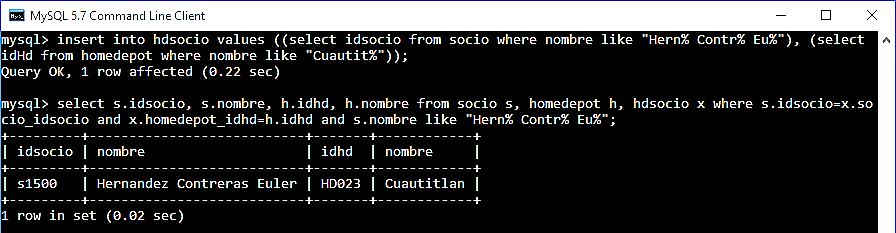
\includegraphics[width=\textwidth]{img/dos.png}
			\label{fig:dos}
		\end{center}
	\end{figure}
	
	El siguiente ejercicio fue cambiar el no. de tel de aquellas sucursales que tienes los siguientes C.P. 77500, 21370. Lo cual se realiza ejecutando las siguientes instrucciones.
	\begin{lstlisting}
	update homedepot
	set tel="55-66-66-66" 
	where direccion like "%77500%" 
	or direccion like "%21370%";
	\end{lstlisting}
	\begin{figure}[H]
		\begin{center}
			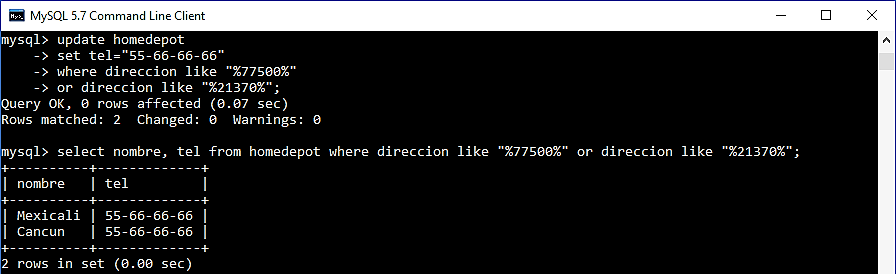
\includegraphics[width=\textwidth]{img/tres.png}
			\label{fig:tres}
		\end{center}
	\end{figure}
	
	El ejercicio tres fue asignar a los asociados que se apellidan GARCIA a otra sucursal.
	\begin{lstlisting}
	select a.nombre, a.homedepot_idhd, h.nombre	from homedepot h, asociado a where a.homedepot_idhd=h.idhd and a.nombre like "%Garc_a%";
	
	update asociado set homedepot_idhd=(select idhd from homedepot where nombre like "%Torres%") where nombre like "%Garc_a%";
	\end{lstlisting}
	\begin{figure}[H]
		\begin{center}
			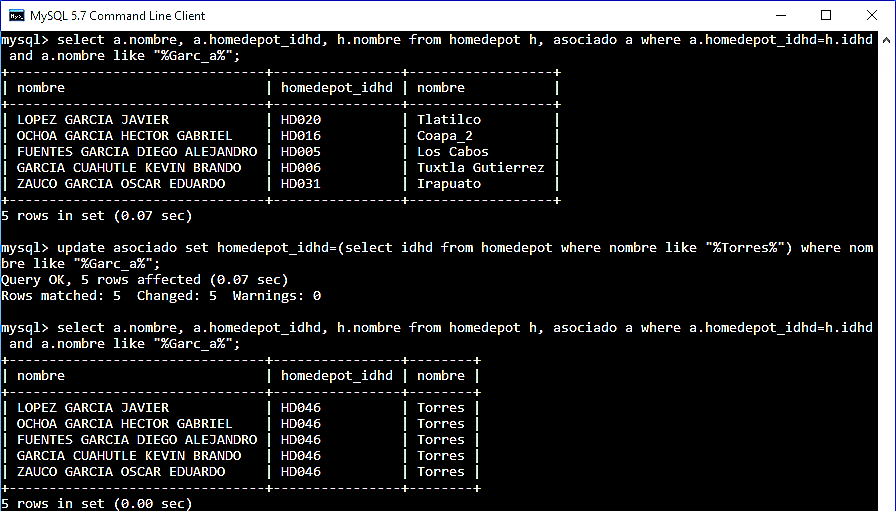
\includegraphics[width=\textwidth]{img/cuatro.png}
			\label{fig:cuatro}
		\end{center}
	\end{figure}
	
	A continuación se agrego el departamento de quejas y se asigno solamente a las sucursales del estado de Jalisco.
	\begin{lstlisting}
	insert into depto values ("D014","QUEJAS"); -- Primero creamos el departamento
	
	-- Luego, buscamos a las sucursales del estado de jalisco
	select idhd, nombre, estado from homedepot where estado like "%Jalisco%";
	
	-- Y procedemos a agregar el departamento a dichas sucursales
	insert into hddepto values ("HD036","D014"),("HD037","D014"), ("HD038","D014");
	\end{lstlisting}
	\begin{figure}[H]
		\begin{center}
			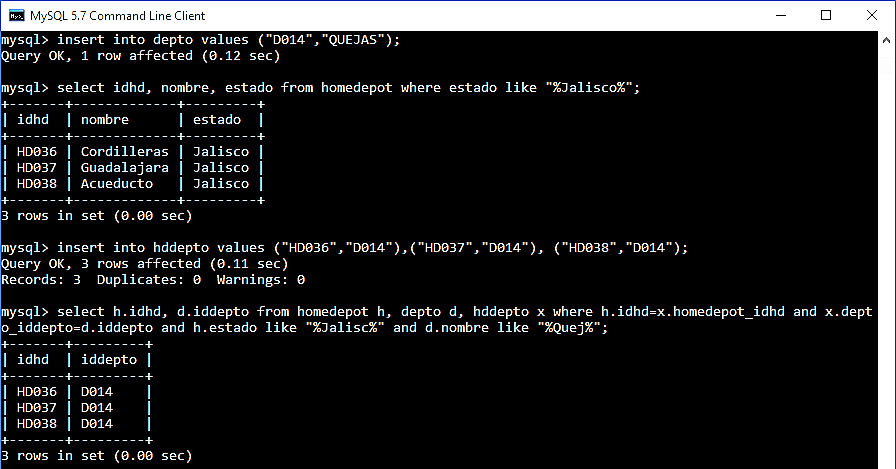
\includegraphics[width=\textwidth]{img/cinco.png}
			\label{fig:cinco}
		\end{center}
	\end{figure}
	
	Finalmente como ultimo ejercicio se eliminaron los socios que se apellidan Ortega.
	\begin{lstlisting}
	select nombre from socio where nombre like "%Ortega%"; --Buscamos a los ortega
	select count(*) from socio; -- Revisamos cuantas tuplas tiene la relacion socio
	delete from socio where nombre like "%Ortega%"; --Borramos a los Ortega
	select count(*) from socio; --Observamos los cambios que han surgido
	\end{lstlisting}
	\begin{figure}[H]
		\begin{center}
			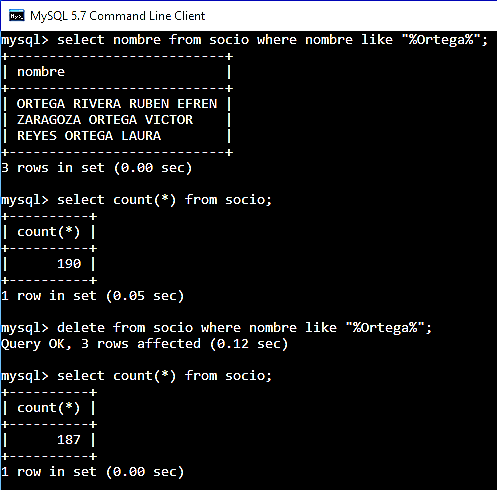
\includegraphics[width=\textwidth]{img/seis.png}
			\label{fig:seis}
			\caption{Eliminación de elementos de la base de datos, se puede observar como cambia el número de socios}
		\end{center}
	\end{figure}
	\section{Conclusiones}
	Esta práctica fue una buena introducción para el manejo de la información de una base de datos, con esto ya no solo se podrán hacer consultas a datos ya establecidos en la base de datos si no que ahora se podrá insertar información que sea necesaria guardar o modificar lo que ya existe en dicha base. Por lo que al juntar esto y las consultas se lograra un manejo de los datos más completo.
	\bibliography{bibliografia} 
	\bibliographystyle{ieeetr}
\end{document}